%%=============================================================================
%% Inleiding
%%=============================================================================

\chapter{\IfLanguageName{dutch}{Inleiding}{Introduction}}%
\label{ch:inleiding}

Lezen is een dagelijkse activiteit voor iedereen. Deze vaardigheid strekt zich uit tot elk aspect van het leven. Dit geldt des te meer in het onderwijs, waar leerkrachten divers leesmateriaal gebruiken om lesinhouden op een authentieke manier over te brengen. Zo zetten leerkrachten in de derde graad van het middelbaar onderwijs wetenschappelijke artikelen in als leesvoer. Toch brengt hun leesgraad een nieuwe uitdaging mee voor zowel scholieren als leerkrachten. 

\medspace

Om scholieren attent te maken van wetenschappelijk onderzoek, lanceerde het Amerikaanse onderwijs het C.R.E.A.T.E.\footnote{https://teachcreate.org/}-initiatief. Het zet twaalf- tot achttienjarige scholieren aan om wetenschappelijke artikelen te lezen in plaats van enkel boeken. Zo begrijpen ze hoe wetenschappers onderzoek plannen, uitvoeren, en resultaten analyseren en interpreteren. Hoewel er geen vergelijkbare Vlaamse initiatieven bestaan, benadrukken de lerarenopleidingen toch het gebruik van afwisselende leerstof in klas. Andere initiatieven, zoals het M-decreet en de leerplannen van het katholiek\footnote{https://pro.katholiekonderwijs.vlaanderen/basisoptie-stem/ondersteunend-materiaal} en het gemeenschapsonderwijs\footnote{https://g-o.be/stem/}, adviseren Vlaamse leerkrachten om hun lessen op een toegankelijke manier aanbieden. Zo nemen zij alle scholieren ongeacht eventuele leesachterstand mee in het verhaal.

\medspace

Met een jaarlijks budget van 32 miljoen euro is Vlaanderen een pionier in Europa op het gebied van artificiële intelligentie (AI) op de werkvloer \autocite{Crevits2022}. Zo stampte de Vlaamse overheid verschillende  projecten uit de grond om Vlaamse AI ontwikkelingen te ondersteunen en AI softwarebedrijven te inspireren. Het amai!-project\footnote{https://amai.vlaanderen/} brengt AI softwarebedrijven uit diverse domeinen samen, waaronder het onderwijs. Zij doelen op een automatisering van processen om de werkdruk bij leerkrachten te verminderen. Dit gebeurt onder andere door \textit{real-time} ondertiteling in de klas en een taalassistent voor leerkrachten in meertalige klasgroepen.


\section{\IfLanguageName{dutch}{Probleemstelling}{Problem Statement}}%
\label{sec:probleemstelling}

De geletterdheid van scholieren bevindt zich op een kritieke punt. Elke drie jaar nemen experts uit 79 geïndustrialiseerde landen de PISA-test af bij middelbare scholen om de leesvaardigheid en wetenschappelijke geletterdheid van 15-jarige scholieren te meten. Uit de PISA-test van 2018 blijkt dat deze doelgroep in Vlaanderen zich echter negatief uit over leesplezier en daarmee de slechtst scorende doelgroep is van alle bevraagde landen. Zoals aangegeven in figuur \ref{img:oeso-leesplezier}, beschouwt bijna de helft van de bevraagden begrijpend lezen als tijdverspilling. Slechts 17\% beschouwt lezen als een hobby. Dit is een dalende trend, want voordien lag dit cijfer hoger dan 20\%. Lezen kan daarmee een obstakel vormen bij deze doelgroep.

\begin{figure}[H]
	\begin{center}
		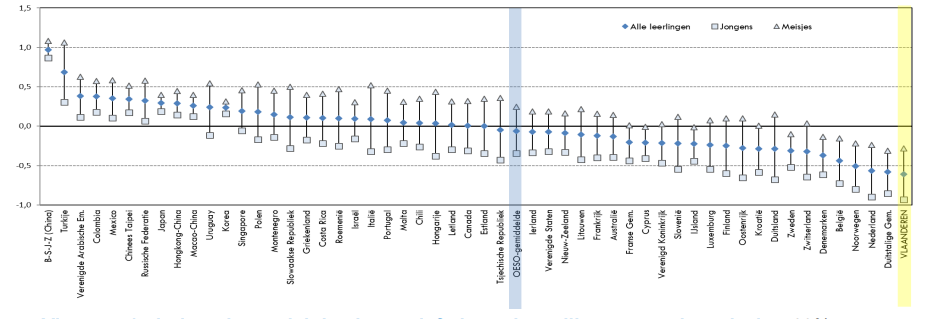
\includegraphics[width=\linewidth]{img/oeso-graphic-leesplezier.png}
	\end{center}
	\caption{Het leesplezier bij 15-jarigen volgens de PISA-test \autocite{DeMeyer2019}.}
	\label{img:oeso-leesplezier}
\end{figure}

Begrijpend lezen valt niet te omzeilen in onze huidige samenleving, maar het leesbegrip verschilt sterk onder studenten in het middelbaar onderwijs. Zo benadrukt \textcite{Vlaanderen2020} dat begrijpend lezen een essentiële vaardigheid is, ook voor vakken buiten Nederlands. Bij wiskunde is begrijpend lezen van cruciaal belang bij complexe vraagstukken. Ook helpt begrijpend lezen studenten om STEM-vakjargon beter te begrijpen.

\medspace 

In het bijzonder hebben scholieren met dyslexie problemen met begrijpend lezen. Onderzoeken van \textcite{Bonte2020, VanDerMeer2022} schatten dat ongeveer 15\% van de Vlaamse scholieren in het middelbaar onderwijs een vorm van dyslexie heeft. Scholieren met dyslexie ervaren moeite en hinder bij het lezen en spellen. Ondanks de bestaande ondersteuning blijven ze toch nog steeds de negatieve impact van hun leerstoornis ervaren. De gevolgen hiervan  kunnen zich doorzetten na het middelbaar onderwijs \autocite{Lissens2020}. Leesvaardigheid blijft daarmee cruciaal voor succes op school en in het werkveld. Scholieren met dyslexie hebben moeilijkheden met deze vaardigheid, wat kan leiden tot onzekerheid en stress. Daarnaast zijn vooroordelen nog steeds een probleem en kunnen ze leiden tot stigmatisering. Echter toont onderzoek aan dat scholieren met dyslexie een sterke doorzettingsvermogen hebben en goede probleemoplossers zijn \autocite{Ghesquiere2018, Lissens2020, Bonte2020}. 

\medspace

Het leerplan voor STEM-vakken stimuleert het gebruik van wetenschappelijke artikelen, maar houdt niet altijd rekening met de bijhorende en complexe leesgraad. De ingewikkelde woordenschat en syntax in wetenschappelijke artikelen kunnen een hindernis vormen voor de begrijpelijkheid van een tekst, aldus \textcite{PlavenSigray2017}. Wetenschappelijke artikelen handmatig vereenvoudigen kan planning, tijd en energie van leerkrachten in het middelbaar onderwijs opslorpen. Het Vlaamse onderwijssysteem staat onder druk en docenten hebben moeite om boven water te blijven. 

\medspace

AI-technologieën zijn vandaag voldoende hoogstaand om tekstvereenvoudiging te automatiseren en om een baanbrekende oplossing te bieden aan het middelbaar onderwijs \autocite{Belpaeme2018}. Het onderwijst past echter zelden soortgelijke technologieën toe. Er is terughoudendheid door enerzijds ouders van leerlingen volgens \textcite{Martens2021a}, anderzijds door de weinige ontwikkelingen in schoolgerelateerde AI-software. Dit terwijl AI-ondersteuning in het onderwijs wel degelijk een positief effect heeft \autocite{Kraft2020}. Er is nood aan een intuïtieve en gebruikersvriendelijke toepassing die taalmodellen of API's kan integreren en aanpassen naargelang de specifieke behoeften van een student met dyslexie. Zo kan dit enerzijds de werkdruk bij leerkrachten verminderen, en anderzijds scholieren in de derde graad ondersteunen bij het lezen van complexe wetenschappelijke artikelen.

\section{\IfLanguageName{dutch}{Onderzoeksvraag}{Research question}}%
\label{sec:onderzoeksvraag}

Dit onderzoek beschrijft het gebruik van AI in de vorm van tekstvereenvoudiging, als advies voor implementatie in het onderwijs. Specifiek om scholieren met dyslexie in de derde graad van het middelbaar onderwijs te ondersteunen bij het begrijpend lezen van wetenschappelijke artikelen. Hiervoor stelt het onderzoek de volgende onderzoeksvraag op: 

\begin{itemize}
	\item Hoe kan een wetenschappelijk artikel automatisch vereenvoudigd worden, gericht op de unieke noden van scholieren met dyslexie in de derde graad middelbaar onderwijs?
\end{itemize}

De oplossingen voor de volgende deelvragen vormen een globaal antwoord op de onderzoeksvraag:

\begin{enumerate}
	% 1
	\item Welke specifieke noden hebben scholieren met dyslexie van de derde graad middelbaar onderwijs bij het begrijpen van complexere teksten? Aanvullend hierop: 
	\begin{itemize}
		\item Wat zijn de specifieke kenmerken van wetenschappelijke artikelen?
	\end{itemize} 
	% 2
	\item Welke aanpakken zijn er voor tekstvereenvoudiging?
	\begin{itemize}
		\item Hoe verloopt de handmatige vereenvoudiging van teksten voor scholieren met dyslexie?
		\item Welke toepassingen, tools en modellen zijn er beschikbaar om Nederlandse geautomatiseerde tekstvereenvoudiging met AI mogelijk te maken?
		\item Hoe is de combinatie van geautomatiseerde tekstvereenvoudiging met gepersonaliseerde  tekstvereenvoudiging mogelijk?
	\end{itemize}
	%4 
	\item Welke functies ontbreken AI-toepassingen om geautomatiseerde tekstvereenvoudiging mogelijk te maken voor scholieren met dyslexie in de derde graad middelbaar onderwijs? 
	\begin{itemize}
		\item Welke manuele methoden voor tekstvereenvoudiging ontbreken in deze tools?
	\end{itemize}
	%3 
	\item Met welke valkuilen bij taalverwerking met AI moeten ontwikkelaars rekening houden?
	% 5
	\item Welk taalmodel of LLM is geschikt voor de ATS van wetenschappelijke artikelen voor scholieren met dyslexie in de derde graad van het middelbaar onderwijs, met dezelfde of gelijkaardige kwaliteiten als gepersonaliseerde MTS?
	% 6
	\item Wat zijn de nodige stappen bij de ontwikkeling van een intuïtieve lokale webtoepassing die zowel scholieren met dyslexie als leerkrachten helpt?
\end{enumerate}


\section{\IfLanguageName{dutch}{Onderzoeksdoelstelling}{Research objective}}%
\label{sec:onderzoeksdoelstelling}

Het onderzoek achterhaalt de technologische en logopedische aspecten waarmee ontwikkelaars rekening meoten houden bij AI-tekstvereenvoudiging. Het resultaat dient als een houvast om hen te begeleiden tijdens de ontwikkeling van deze applicaties voor gepersonaliseerde en geautomatiseerde tekstvereenvoudiging. Verder ontwikkelt het onderzoek een soortgelijke toepassing in het bijzonder voor scholieren met dyslexie in de derde graad van het middelbaar onderwijs. Dit resulteert in een uitgewerkt prototype voor tekstvereenvoudiging, genaamd \textit{Pentimentor}. \textit{Pentimentor} heeft voornamelijk twee functies. Allereerst kan \textit{Pentimentor} wetenschappelijke artikelen vereenvoudigen op basis van de specifieke behoeften van scholieren met dyslexie in de derde graad van het middelbaar onderwijs. Daarnaast biedt \textit{Pentimentor} een geautomatiseerde benadering om wetenschappelijke artikelen op een gepersonaliseerde manier te vereenvoudigen door het gebruik van aanpasbare parameters. Tot slot geeft \textit{Pentimentor} de eindgebruiker het vereenvoudigd artikel terug in Word-formaat. 

\section{\IfLanguageName{dutch}{Opzet van deze bachelorproef}{Structure of this bachelor thesis}}%
\label{sec:opzet-bachelorproef}

De rest van deze scriptie is als volgt opgebouwd:

\begin{itemize}
	\item Hoofdstuk~\ref{ch:stand-van-zaken} geeft een overzicht van de stand van zaken binnen het onderzoeksdomein, op basis van een literatuurstudie.
	\item Hoofdstuk~\ref{ch:methodologie} licht de methodologie toe. Het onderzoek vermeldt de gebruikte onderzoekstechnieken om een antwoord te kunnen formuleren op de onderzoeksdeelvragen. 
	\item Hoofdstuk~\ref{ch:resultaten} bevat de resultaten voor alle onderzoekstechnieken.
	\item Hoofdstuk~\ref{ch:conclusie} geeft de uiteindelijke conclusie en beantwoordt daarmee de onderzoeksvraag.
	\item Tot slot geeft hoofdstuk~\ref{ch:discussie} verdere aanbevelingen en aanzet voor toekomstig onderzoek binnen de bestudeerde domeinen. 
\end{itemize}
